%%
%% Toolbox Language Manual
%% $Id: m4lib.tex,v 1.33 2006/04/19 10:25:12 vdmtools Exp $
%% 

%%%%%%%%%%%%%%%%%%%%%%%%%%%%%%%%%%%%%%%%
% PDF compatibility code. 

\makeatletter
\newif\ifpdflatex@
\ifx\pdftexversion\@undefined
\pdflatex@false
%\message{Not using pdf}q
\else
\pdflatex@true
%\message{Using pdf}
\fi

\newcommand{\latexpdf}[2]{
  \ifpdflatex@ #1
  \else #2
  \fi
}

\newcommand{\latexorpdf}[2]{
  \ifpdflatex@ #2
  \else #1
  \fi
}

\makeatother

#ifdef A4Format
\newcommand{\pformat}{a4paper}
#endif A4Format
#ifdef LetterFormat
\newcommand{\pformat}{letterpaper}
#endif LetterFormat

%%%%%%%%%%%%%%%%%%%%%%%%%%%%%%%%%%%%%%%%

\latexorpdf{
\documentclass[\pformat,12pt]{jarticle}
}{
% pdftex option is used by graphic[sx],hyperref,toolbox.sty
\documentclass[\pformat,pdftex,12pt]{jarticle}
}

\usepackage{toolbox}
\usepackage{rotating}
\usepackage{verbatimfiles}
\usepackage{alltt}
%\usepackage{path}
\usepackage{longtable}

% Ueki change start
\usepackage[dvipdfm,bookmarks=true,bookmarksnumbered=true,colorlinks,plainpages=true]{hyperref}
% Ueki change end

% Ueki delete start
%\latexorpdf{
%\usepackage[plainpages=true,colorlinks,linkcolor=black,citecolor=black,pagecolor=black, urlcolor=black]{hyperref}
%}{
%\usepackage[plainpages=true,colorlinks]{hyperref}
%}
% Ueki delete end

%\floatstyle{plain}
%\restylefloat{figure}
\AtBeginDvi{\special{pdf:tounicode 90ms-RKSJ-UCS2}}
\newcommand{\VDM}{VDM++}

\def\insertfig#1#2#3#4{ % Filename, width, caption, label
\begin{figure}[htb]
\begin{center}
\resizebox{#2}{!}{\includegraphics{#1}}
\end{center}
\caption{#3} #4
\end{figure} 
}


\begin{document}

\vdmtoolsmanualcsk{VDM C++ ライブラリ}
       {v9.0.6}
       {2016}
       {VDM++}
       {1.0}

\section{導入}

本書では、VDM C++ ライブラリを構成するクラスとメソッドの記述を行う。
本書を読むためには、いくらかの C++ の知識が必要となる。
各々 VDM 型に対して、その型を実装する相当する C++ クラスが1つ存在する。
加えて合成型に対しては、VDM C++ ライブラリには集合、写像、列のテンプレートがあり、更に良質な型情報を含む型宣言を可能にしている。

第 \ref{conventions}章で、本書で使用する表記法が一覧されている。
第 \ref{general-structure}章では、VDM オブジェクトの一般的構造を簡単に示す。
第\ref{general-op} 章ですべての VDM クラスに共通する関数を記述し、他方では第 \ref{specific-op}章で各々 VDM クラスにおいて実行可能な特有関数が一覧されている。 
集合、写像、列のためのテンプレートは、第\ref{templates}章に記されている。
第\ref{error-messages}章には、全エラーメッセージを記述する。

付録 \ref{files} には、VDM C++ ライブラリを構成するファイルが一覧されている。

ライブラリの最新版は次のプラットフォーム上で利用可能である:
\begin{itemize}
\item Microsoft Windows 2000/XP/Vista上のMicrosoft Visual C++ 2005 SP1
\item Mac OS X 10.4, 10.5
\item Linux Kernel 2.4, 2.6上のGNU gcc 3, 4
\item Solaris 10
\end{itemize}


\section{表記法} 
\label{conventions}
本書では以下の慣例を用いる:

\vspace{0.5cm}

\begin{center}
\begin{longtable}{|c|l|l|} 
\hline
{\em 変数名} & {\em 変数型} & {\em C++ クラス} \\ \hline \hline
\endhead
\hline
\endfoot
{\tt i} & C++ 整数型 & {\tt int}\\
{\tt c} & C++ 文字型 & {\tt char}\\
{\tt d} & C++ ダブル型 & {\tt double}\\
{\tt s} & C++ 文字列型 & {\tt string}\\
{\tt I} & VDM 整数型  & {\tt Int}\\
{\tt M} & VDM 写像型 & {\tt Map}\\
{\tt C} & VDM 文字型 & {\tt Char}\\
{\tt B} & VDM ブール型 & {\tt Bool}\\
{\tt N} & VDM Nil型 & {\tt Nil}\\
{\tt Q} & VDM 引用型 & {\tt Quote}\\
{\tt G} & VDM 汎用型 & {\tt Generic}\\
{\tt Rl} & VDM 実数型 & {\tt Real}\\
{\tt Rc} & VDM レコード型 & {\tt Record}\\
{\tt Tx} & VDM テキスト型 & {\tt Text}\\
{\tt Tp} & VDM 組型 & {\tt Tuple}\\
{\tt Tk} & VDM トークン型 & {\tt Token}\\
{\tt St} & VDM 集合型 & {\tt Set}\\
{\tt Sq} & VDM 列型 & {\tt Sequence}\\ 
{\tt Ob} & VDM オブジェクト参照型 & {\tt ObjectRef}\\ 
{\tt A} & 上記 VDM 型のいずれか &\\
\end{longtable}
\end{center}


\section{VDM 値の一般的構造} \label{general-structure}

この章では、``水面下''でどのようなことが行われているかの考え方を示すため、VDM値の一般的構造を簡単に述べていく。
 VDM C++ クラスを用いるには、このようなある程度の基本的知識をもつことが重要である。

\begin{figure}[!hbt]
\begin{center}
\resizebox{8cm}{!}{\includegraphics{fig1}}
%\includegraphics{fig1}
\caption{一般的構造\label{fig1}}
\end{center}
\end{figure}

{\tt Set}、{\tt Int}、{\tt Map}等のVDMクラスすべてに対して、{\tt SetVal}、{\tt IntVal}、{\tt MapVal} 等という名称をもつ相当する値クラスが1つずつ存在する。
すべての VDM クラスは {\tt Common}クラスのサブクラスで、一方すべての値クラスは {\tt MetaivVal}クラスのサブクラスである。

たとえば変数 {\tt I}が {\tt Int}型で宣言されているならば、{\tt Int}型と {\tt IntVal} 型のインスタンスが生成され{\tt Int} インスタンスからの ポインタ {\tt p}  (このポインタは実際には {\tt Common}で定義される) が {\tt IntVal}インスタンス(実際には {\tt IntVal}インスタンスの {\tt MetaivVal}部分)を指し示している。
この状態は図\ref{fig1}で描かれている。
破線はクラス階層を表し、実線はポインタ {\tt p}を示す。 
{\tt I}の値は {\tt IntVal} インスタンス中に置かれている。
以降で、変数値の参照とは常に、ポインタ {\tt p}が指し示す Valクラスのインスタンスを意味する。

\begin{figure}[hbt]
  \begin{center}
    \includegraphics{fig2}
    \caption{汎用クラス\label{fig2}}
  \end{center}
\end{figure}


合併型の考え方をサポートするものとして、 {\tt 汎用}クラスが導入されている。
これは合成 VDM 型 ({\tt 写像、列、組、集合、レコード}) を示すクラスのインスタンスが、同時に異なる型の要素を含めることを許す。
汎用値としては、基本の{\tt IntVal,RealVal} から{\tt TupleVal, SequenceVal}といった合成値まで任意の VDM 値であってよい。
このことは、 {\tt 汎用}型の変数は任意の VDM 型の基礎となる値を含めることが可能であることを意味する。
図\ref{fig2} では汎用の例題を2つ示す。

現実には、合成型は{\tt 汎用}型の要素だけを含めることができるように実装されている。
合成型に要素を挿入する関数のほとんどは、挿入前に要素を自動的に {\tt 汎用}型にキャストすることができるが、要素を取り出す関数は常に {\tt 汎用}型を返す。

この例を示すために VDM 式を見てみよう:

\begin{verbatim}
let Sq = [1,<TWO>] in
  ...
\end{verbatim}

列 {\tt Sq} は整数と引用の両方を含む。
 C++ が強く型付けされているので、 let-式の C++ 実装では、 {\tt Generic} に対する整数と引用のキャストを、列 {\tt Sq}に追加する前に行わなければならない。
以下の実装において、このキャストは {\tt ImpAppend} 関数により自動的になされ、取り出し関数である{\tt Hd()}は {\tt Generic}を返す。 
この列の最初の要素は {\tt Int}型なので、その後 {\tt G} は {\tt Int}にキャストすることができる。 

\begin{verbatim}
Sequence Sq;  Generic G;

Sq.ImpAppend(Int(1)); 
Sq.ImpAppend(Quote(``<TWO>''));

G = Sq.Hd();
\end{verbatim}

一般的にはどのような型も {\tt Generic}にキャストされることは可能であるが、汎用であるのは表面上のみであり、基礎となる値は保持されている。
たとえば、図\ref{fig2} 上の汎用 {\tt G1} は後から逆のキャストで {\tt Int}にもどすことが可能である。合成型 ({\tt 写像、列、組、集合、レコード}) を表わすすべてのクラスに対して、そのクラスに含まれるすべての要素が含まれる前に自動的に {\tt Generic}にキャストされる。
これは、合成変数から要素が取り出されるときは常に {\tt Generic}型になることを意味する。
必要ならば、元の型へ逆キャストを行うことも可能である。


\section{VDM 型の一般関数} 
\label{general-op}

この章では、 {\tt Common} クラスで定義されているすべての型のインスタンスに適用可能な全ての関数を記述する。
\footnote{VDMTools内部の文字コードはUnicodeを使用しているため、VDM型とwstringを交換する場合、文字コードに注意する。}
\subsection*{関数}

\begin{description}
\item[{\tt A.MyValType()}] \mbox{}\\
     {\tt A}の値の型を返す。

     結果型 : {\bf metaivType}
     
     \vspace{1cm}
     列挙型 {\tt metaivType} がライブラリの一部であることに注意する。

\begin{quote}
\begin{verbatim}
enum metaivType {
  mt_nil, mt_char, mt_int, mt_real, mt_quote,
  mt_tuple, mt_record, mt_set, mt_map, mt_generic,
  mt_text, mt_token, mt_bool, mt_sequence, 
  mt_objectref, mt_undef
}
\end{verbatim}
\end{quote}

\item[{\tt A1 = A2}] \mbox{}\\
     {\tt A1} に {\tt A2}の値を与える。
{\tt A1} が{\tt Generic}型であるならば、 {\tt A2} は任意の型の可能性がある。
この場合、 {\tt A1} はそのまま汎用型であるが {\tt A2}の値を含むことになる。
それ以外の場合は、 {\tt A2} の値の型は {\tt A1}の値の型と同じでなければならない。

結果型 : A1への参照 
     
\item[{\tt A1 == A2}] \mbox{}\\
  {\tt A1}の値が {\tt A2}の値と等しければ {\tt true} を返し、それ以外は {\tt false} を返す。

     結果型 : {\bf bool}

\item[{\tt A1 != A2}] \mbox{}\\
  {\tt A1}の値が {\tt A2}の値と等しくなければ {\tt true} を返し、それ以外は {\tt false} を返す。

     結果型 : {\bf bool}

\item[{\tt A.ascii()}] \mbox{}\\
  VDM 値の ASCII表現を含む {\tt 文字列} を返す。

     結果型 : {\bf wstring}
     
\item[{\tt A.IsNil()}] \mbox{}\\
     {\tt A} の値が {\tt Nil}型であるならば {\tt true} を返す

     結果型 : {\bf bool}
     
\item[{\tt A.IsChar()}] \mbox{}\\
     {\tt A} が {\tt Char}型であるならば{\tt true}を返す

     結果型 : {\bf bool}

\item[{\tt A.IsInt()}] \mbox{}\\
      {\tt A} が{\tt Int}型であるならば {\tt true} を返す

     結果型 : {\bf bool}

\item[{\tt A.IsReal()}] \mbox{}\\
      {\tt A} が {\tt Real}型であるならば {\tt true}を返す

     結果型 : {\bf bool}

\item[{\tt A.IsQuote()}] \mbox{}\\
      {\tt A} が {\tt Quote}型であるならば {\tt true} を返す

     結果型 : {\bf bool}

\item[{\tt A.IsTuple()}] \mbox{}\\
      {\tt A} が {\tt Tuple}型であるならば {\tt true} を返す

     結果型 : {\bf bool}

\item[{\tt A.IsRecord()}] \mbox{}\\
     {\tt A} が {\tt Record}型であるならば {\tt true} を返す

     結果型 : {\bf bool}

\item[{\tt A.IsSet()}] \mbox{}\\
     {\tt A} が {\tt Set}型であるならば {\tt true} を返す

     結果型 : {\bf bool}

\item[{\tt A.IsMap()}] \mbox{}\\
     {\tt A} が {\tt Map}型であるならば {\tt true} を返す

     結果型 : {\bf bool}

\item[{\tt A.IsText()}] \mbox{}\\
     {\tt A} が {\tt Text}型であるならば {\tt true} を返す

     結果型 : {\bf bool}

\item[{\tt A.IsToken()}] \mbox{}\\
      {\tt A} が {\tt Token}型であるならば {\tt true} を返す

     結果型 : {\bf bool}

\item[{\tt A.IsBool()}] \mbox{}\\
     {\tt A} が {\tt Bool}型であるならば {\tt true} を返す

     結果型 : {\bf bool}

\item[{\tt A.IsSequence()}] \mbox{}\\
      {\tt A} が {\tt Sequence}型であるならば {\tt true} を返す

     結果型 : {\bf bool}

\item[{\tt A.IsObjectRef()}] \mbox{}\\
     {\tt A} が {\tt ObjectRef}型であるならば {\tt true} を返す

     結果型 : {\bf bool}

\item[{\tt A.WriteVal(o)}] \mbox{}\\
{\tt A} の値を、関数 ReadValを用いて再び値を読み込むことができる形式で {\tt ostream} {\tt o}に書き込む。
  {\tt ReadVal} と {\tt WriteVal} は、ファイルシステムに値を保存するために用いられ、後で読み戻しを行う(永続性)。

  結果型: {\bf void}
  
\item[{\tt Generic g; g = ReadVal(i)}] \mbox{}\\
  (istreamを通して)  WriteVal メソッドで書かれたファイルから 値を読み込む。
 {\tt ReadVal} は関数であり、メソッドではないことに注意する。
  
  {\tt WriteVal} が書き込み {\tt ReadVal} が読み込む形式は低レベルフォーマットであって、人が取り扱うためのものではない。
  
  結果型: {\bf Generic}
\end{description}


\subsection*{例題}

この節で述べられた関数を用いた例題 C++ プログラム。

\begin{verbatim}
    Generic G1;  Int I1(3),I2(4),I3;

    G1 = I1;
    I3 = G1;
    if (G1 == I3)
      wcout << "The value of G1 equals the value of I3" << endl;
    if (G1.IsInt())
      wcout << "The value of G1 is of type Int" << endl;
      wcout << G1.MyValType() << "  The value of G1 is of type Int" << endl;
      wcout << I1.ascii()  << "  The ASCII representation of I1" << endl;
\end{verbatim}

\noindent このプログラムの実行結果は次の通り :

\begin{verbatim}
The value of G1 equals the value of I3
The value of G1 is of type Int
103  The value of G1 is of type Int
3  The ASCII representation of I1
\end{verbatim}

%\noindent 値 {\tt 2} は {\tt mt\_int}に相当する。

\subsection{出力ワイドストリームへ値の印刷}
\label{sec:Printing}

\texttt{os << v}と表すことで任意の VDM 値 \texttt{v} を 出力ワイドストリーム \texttt{os} へ印刷することが可能である。

レコードは、既定では \path+mk_unknown4(...)+ というように、数値タグと共に印刷されることになる。
また、タグ名を文字形式で印刷するには、\ref{The Record Information Map} The Record Information Mapを使用する。
\subsubsection*{例題}
\verbatimfile{tagmap.cc}

\noindent このプログラムの実行結果は次の通り : 
\begin{verbatim}
r1=mk_X`a( 
mk_X`b( 
mk_X`b( 100 ) ) )
\end{verbatim}

\section{VDM 型の特有関数} \label{specific-op}
\subsection{Int}
{\tt Int} は以下の要素関数をサポートしている:

\vspace{0.5cm}

\begin{description}
\item[{\tt Int I}] \mbox{}\\
      {\tt I} を {\tt Int}として宣言する。
{\tt I} の値は 0に初期化される。

     結果型 : {\bf void}
\item[{\tt Int I(i)}] \mbox{}\\
      {\tt I} を {\tt Int}として宣言し、初期値を {\tt i}とする。

     結果型 : {\bf void}

\item[{\tt Int I(I1)}] \mbox{}\\
      {\tt I} を {\tt Int}として宣言し、値は  {\tt I1}と等しいとする。

     結果型 : {\bf void}

\item[{\tt I.GetValue()}] \mbox{}\\
     {\tt I}の C++ 整数値を返す。

     結果型 : {\bf int}

\item[{\tt I = i}] \mbox{}\\
      {\tt i}の値を {\tt I} に与える。

     結果型 : {\bf Int\&}

\item[{\tt -I}] \mbox{}\\
     単項マイナス。{\tt I}の正負逆符号の値をもつ {\tt Int} を返す。

     結果型 : {\bf Int}

\item[{\tt I1 + I2}] \mbox{}\\
     2項加算。 

     結果型 : {\bf Int}

\item[{\tt I + R}] \mbox{}\\
     2項加算。 

     結果型 : {\bf Real}

\item[{\tt I1 - I2}] \mbox{}\\
     2項減算。

     結果型 : {\bf Int}

\item[{\tt I - R}] \mbox{}\\
     2項減算。 

     結果型 : {\bf Real}

\item[{\tt I1 * I2}] \mbox{}\\
     2項乗算。 

     結果型 : {\bf Int}

\item[{\tt I * R}] \mbox{}\\
     2項乗算。 

     結果型 : {\bf Real}

\item[{\tt I1 / I2}] \mbox{}\\
     2項除算。 

     ゼロによる除算はエラー \ 第‾\ref{error-messages}章参照 を起こす。

     結果型 : {\bf Real}

\item[{\tt I / R}] \mbox{}\\
     2項除算。 

     ゼロによる除算はエラー \ 第‾\ref{error-messages}章参照 を起こす。

     結果型 : {\bf Real}

\item[{\tt I1.Exp(I2)}] \mbox{}\\
     指数演算。

     結果型 : {\bf Real}

\item[{\tt I.Exp(R)}] \mbox{}\\
     指数演算。

     結果型 : {\bf Real}

\end{description}

\subsection*{例題}

\begin{verbatim}
    Int I1(3),I2;
    Int I3(I1);

    if (I1 == I3)
      wcout << "The value of I1 equals the value of I3" << endl;
      wcout << I2.GetValue() << "  is the initial value of I2" << endl;
    I2 = 10;
      wcout << I2.GetValue() << "  is the new value of I2" << endl;
\end{verbatim}

\noindent このプログラムの実行結果は以下の通り :

\begin{verbatim}
The value of I1 equals the value of I3
0  is the initial value of I2
10  is the new value of I2
\end{verbatim}


\subsection{Real}
{\tt Real} は以下の要素関数をサポートしている:

\vspace{0.5cm}

\begin{description}
\item[{\tt Real Rl}] \mbox{}\\
     {\tt Rl} を {\tt Real}として宣言する。 
{\tt Rl} の値は 0に初期化される。

     結果型 : {\bf void}

\item[{\tt Real Rl(d)}] \mbox{}\\
      {\tt Rl} を {\tt Real} として宣言し、値に {\tt d}で初期化する。

     結果型 : {\bf void}

\item[{\tt Real Rl(Rl1)}] \mbox{}\\
     {\tt Rl} を {\tt Real} として宣言し、値は {\tt Rl1}に等しい。

     結果型 : {\bf void}

\item[{\tt Rl.GetValue()}] \mbox{}\\
      {\tt Rl}の C++ {\tt double}値を返す。

     結果型 : {\bf double}
     
\item[{\tt Rl = d}] \mbox{}\\
      {\tt Rl} に {\tt d}の値を与える。

     結果型 : {\bf Real\&}

\item[{\tt -R}] \mbox{}\\
     単項マイナス。  {\tt R}の逆符号の値をもつ {\tt Real} を返す。

     結果型 : {\bf Real}

\item[{\tt R1 + R2}] \mbox{}\\
     2項加算。 

     結果型 : {\bf Real}

\item[{\tt R + I}] \mbox{}\\
     2項加算。

     結果型 : {\bf Real}

\item[{\tt R1 - R2}] \mbox{}\\
     2項減算。 

     結果型 : {\bf Real}

\item[{\tt R - I}] \mbox{}\\
     2項減算。 

     結果型 : {\bf Real}

\item[{\tt R1 * R2}] \mbox{}\\
     2項乗算。 

     結果型 : {\bf Real}

\item[{\tt R * I}] \mbox{}\\
     2項乗算。 

     結果型 : {\bf Real}

\item[{\tt R1 / R2}] \mbox{}\\
     2項除算。 

     結果型 : {\bf Real}

\item[{\tt R / I}] \mbox{}\\
     2項除算。 

     結果型 : {\bf Real}

\item[{\tt R1.Exp(R2)}] \mbox{}\\
     指数演算。 

     結果型 : {\bf Real}

\item[{\tt R.Exp(I)}] \mbox{}\\
     指数演算。 

     結果型 : {\bf Real}
\end{description}

\subsection*{例題}

\begin{verbatim}
    Real Rl1(3.2),Rl2;
    Real Rl3(Rl1);

    if (Rl1 == Rl3)
      wcout << "The value of Rl1 equals the value of Rl3" << endl;
      wcout << Rl2.GetValue() << "  is the initial value of Rl2" << endl;
    Rl2 = 10.5;
      wcout << Rl2.GetValue() << "  is the new value of Rl2" << endl;
\end{verbatim}

\noindent このプログラムの実行結果は次の通り :

\begin{verbatim}
The value of Rl1 equals the value of Rl3
0 is the initial value of Rl2
10.5  is the new value of Rl2
\end{verbatim}

\subsection{Bool}
{\tt Bool} は以下の要素関数をサポートする:

\vspace{0.5cm}

\begin{description}
\item[{\tt Bool B}] \mbox{}\\
      {\tt B} を {\tt Bool}として宣言する。 {\tt B} の値は 0 ({\tt false})に初期化される。 

     結果型 : {\bf void}

\item[{\tt Bool B(i)}] \mbox{}\\
     {\tt B} を {\tt Bool} として宣言し、値は {\tt i}に初期化する。

     結果型 : {\bf void}

\item[{\tt Bool B(B1)}] \mbox{}\\
     {\tt B} を {\tt Bool} として宣言し、値は {\tt B1}に等しい。

     結果型 : {\bf void}

\item[{\tt B.GetValue()}] \mbox{}\\
     {\tt B}の C++ {\bf bool}値を返す。

     結果型 : {\bf bool}

\item[{\tt B = i}] \mbox{}\\
     {\tt i}の値を {\tt B} に与える。

     結果型 : {\bf Bool\&}

\item[{\tt B.mnot()}] \mbox{}\\
     論理否定。

     結果型 : {\bf Bool}

\item[{\tt !B}] \mbox{}\\
     論理否定。

     結果型 : {\bf Bool}

\item[{\tt B1.mand(B2)}] \mbox{}\\
     論理積。

     結果型 : {\bf Bool}

\item[{\tt B1 \&\& B2}] \mbox{}\\
     論理積。

     結果型 : {\bf Bool}

\item[{\tt B1.mor(B2)}] \mbox{}\\
     論理和。

     結果型 : {\bf Bool}

\item[{\tt B1 || B2}] \mbox{}\\
     論理和。

     結果型 : {\bf Bool}

\end{description}

\subsection*{例題}

\begin{verbatim}
    Bool B1(3),B2;
    Bool B3(B1);

    if (B1 == B3)
      wcout << "The value of B1 equals the value of B3" << endl;
      wcout << B2.GetValue() << "  is the initial value of B2" << endl;
    B2 = true;
      wcout << B2.GetValue() << "  is the new value of B2 (true)" << endl;
\end{verbatim}

\noindent この実行プログラムの結果は次の通り :

\begin{verbatim}
    The value of B1 equals the value of B3
    0  is the initial value of B2
    1  is the new value of B2 (true)
\end{verbatim}


\subsection{Nil}
{\tt Nil} は以下の要素関数をサポートする:

\vspace{0.5cm}

\begin{description}
\item[{\tt Nil N}] \mbox{}\\
     {\tt N} を {\tt Nil}型の値として宣言する。

     結果型 : {\bf void}

\end{description}

\noindent  {\tt Nil} 型のインスタンスは全型に共通の関数のみをサポートする (第 \ref{general-op}章を参照)。


\subsection{Quote}
{\tt Quote} は以下の要素関数をサポートする:

\vspace{0.5cm}

\begin{description}
\item[{\tt Quote Q}] \mbox{}\\
      {\tt Q} を {\tt Quote}型の値として宣言する。 {\tt Q}の値は {\tt ""}に初期化される。

     結果型 : {\bf void}

\item[{\tt Quote Q(s)}] \mbox{}\\
      {\tt Q} を {\tt Quote} 型の値として宣言し、値を {\tt s}に初期化する。

     結果型 : {\bf void}

\item[{\tt Quote Q(Q1)}] \mbox{}\\
      {\tt Q} を、{\tt Q1}と等しい {\tt Quote} 型の 値として宣言する。

     結果型 : {\bf void}

\item[{\tt Q.GetValue()}] \mbox{}\\
      {\tt Q}の C++ ワイド文字列値を返す。

     結果型 : {\bf wstring}

\item[{\tt Q = s}] \mbox{}\\
      {\tt s}の値を {\tt Q} に与える。

     結果型 : {\bf Quote\&}
\end{description}

\subsection*{例題}

\begin{verbatim}
    Quote Q1(L"Q_ONE"),Q2;
    Quote Q3(Q1);

    if (Q1 == Q3)
      wcout << "The value of Q1 equals the value of Q3" << endl;
      wcout << Q2.GetValue() << "  is the initial value of Q2" << endl;
    Q2 = L"Q_TWO";
      wcout << Q2.GetValue() << "  is the new value of Q2" << endl;
\end{verbatim}

\noindent このプログラムの実行結果は次の通り :

\begin{verbatim}
    The value of Q1 equals the value of Q3
      is the initial value of Q2
    Q_TWO  is the new value of Q2
\end{verbatim}


\subsection{Char}
{\tt Char} は以下の要素関数をサポートする:

\vspace{0.5cm}

\begin{description}
\item[{\tt Char C}] \mbox{}\\
      {\tt C} を {\tt Char}型の値として宣言する。 {\tt C}の値は {\tt '?'}に初期化される。

     結果型 : {\bf void}

\item[{\tt Char C(c)}] \mbox{}\\
      {\tt C} を {\tt Char} 型の値として宣言し、値を {\tt c}と初期化する。

     結果型 : {\bf void}

\item[{\tt Char C(C1)}] \mbox{}\\
      {\tt C} を、{\tt C1}と等しい {\tt Char} 型の値として宣言する。

     結果型 : {\bf void}

\item[{\tt C.GetValue()}] \mbox{}\\
     {\tt C}のC++ ワイド文字値を返す。

     結果型 : {\bf wchar\_t}
     
\item[{\tt C = c}] \mbox{}\\
     {\tt C} に {\tt c}の値を与える。

     結果型 : {\bf Char\&}
\end{description}

\subsection*{例題}

\begin{verbatim}
    Char C1(L'c'),C2;
    Char C3(C1);

    if (C1 == C3)
      wcout << "The value of C1 equals the value of C3" << endl;
      wcout << C2.GetValue() << "  is the initial value of C2" << endl;
    C2 = L'd';
      wcout << C2.GetValue() << "  is the new value of C2" << endl;
\end{verbatim}

\noindent このプログラムの実行結果は次の通り :

\begin{verbatim}
    The value of C1 equals the value of C3
    ?  is the initial value of C2
    d  is the new value of C2
\end{verbatim}


\subsection{Text}
{\tt Text} は以下の要素関数をサポートする:

\vspace{0.5cm}

\begin{description}
\item[{\tt Text Tx}] \mbox{}\\
      {\tt Tx} を {\tt Text}型の値として宣言する。 {\tt Tx}の値は {\tt ""}に初期化される。

     結果型 : {\bf void}

\item[{\tt Text Tx(s)}] \mbox{}\\
      {\tt Tx} を {\tt Text}型 の値として宣言し、値を {\tt s}に初期化する。

     結果型 : {\bf void}

\item[{\tt Text Tx(Tx1)}] \mbox{}\\
      {\tt Tx} を、{\tt Tx1}と等しい値を持つ {\tt Text}型 の値として宣言する。

     結果型 : {\bf void}

\item[{\tt Tx.GetValue()}] \mbox{}\\
      {\tt Tx}の C++ ワイド文字列値を返す。

     結果型 : {\bf wstring}

\item[{\tt Tx = s}] \mbox{}\\
     {\tt Tx} に {\tt s}の値を与える。

     結果型 : {\bf Text\&}
\end{description}

\subsection*{例題}

\begin{verbatim}
    Text Tx1(L"Tx_ONE"),Tx2;
    Text Tx3(Tx1);

    if (Tx1 == Tx3)
      wcout << "The value of Tx1 equals the value of Tx3" << endl;
      wcout << Tx2.GetValue() << "  is the initial value of Tx2" << endl;
    Tx2 = L"Tx_TWO";
      wcout << Tx2.GetValue() << "  is the new value of Tx2" << endl;
\end{verbatim}

\noindent このプログラムの実行結果は次の通り :

\begin{verbatim}
    The value of Tx1 equals the value of Tx3
      is the initial value of Tx2
    Tx_TWO  is the new value of Tx2
\end{verbatim}


\subsection{Token}
{\tt Token} は以下の要素関数をサポートする:

\vspace{0.5cm}

\begin{description}
\item[{\tt Token Tk}] \mbox{}\\
      {\tt Tk} を {\tt Token}型の値として宣言する。 {\tt Tk}の値は {\tt ""}に初期化されている。

     結果型 : {\bf void}

\item[{\tt Token Tk(s)}] \mbox{}\\
      {\tt Tk} を {\tt Token} 型の値として宣言し、値を {\tt s}に初期化する。

     結果型 : {\bf void}

\item[{\tt Token Tk(Tk1)}] \mbox{}\\
      {\tt Tk} を{\tt Tk1}と等しい {\tt Token}型 の値として宣言する。

     結果型 : {\bf void}

\item[{\tt Tk.GetValue()}] \mbox{}\\
      {\tt Tk}の C++ ワイド文字列値を返す。

     結果型 : {\bf wstring}

\item[{\tt Tk = s}] \mbox{}\\
      {\tt Tk} に {\tt s}の値を与える。

     結果型 : {\bf Token\&}
\end{description}

\subsection*{例題}

\begin{verbatim}
    Token Tk1(L"Tk_ONE"),Tk2;
    Token Tk3(Tk1);

    if (Tk1 == Tk3)
      wcout << "The value of Tk1 equals the value of Tk3" << endl;
      wcout << Tk2.GetValue() << "  is the initial value of Tk2" << endl;
    Tk2 = L"Tk_TWO";
      wcout << Tk2.GetValue() << "  is the new value of Tk2" << endl;
\end{verbatim}

\noindent このプログラムの実行結果は次の通り :

\begin{verbatim}
    The value of Tk1 equals the value of Tk3
      is the initial value of Tk2
    Tk_TWO  is the new value of Tk2
\end{verbatim}




\subsection{Map}
{\tt Map} は以下の要素関数をサポートする:

\vspace{0.5cm}

\begin{description}
\item[{\tt Map M}] \mbox{}\\
     {\tt M} を {\tt Map} 型の値として宣言し、空写像に初期化する。

     結果型 : {\bf void}

\item[{\tt Map M(M1)}] \mbox{}\\
      {\tt M} を {\tt Map} 型の値として宣言し、 {\tt M1}に初期化する。

     結果型 : {\bf void}

\item[{\tt M.Insert(A1, A2)}] \mbox{}\\
キー {\tt A1} をそれに伴う内容 {\tt A2}と共に {\tt M}に挿入する。 
キー {\tt A1}がすでに {\tt M} の定義域に属している場合は、 A2 が値域値と等しいかどうかがチェックされる。
  等しくなければ、エラー \ 第‾\ref{error-messages}章参照 が起こされる。 
  関数は {\tt M}への参照を返す。

     結果型 : {\bf Map\&}

\item[{\tt M.ImpModify(A1, A2)}] \mbox{}\\
     キー {\tt A1}が {\tt M} の定義域に既に属しているならば値域値が {\tt A2}に変更されるということを除けば、 {\tt Insert} として作用する。 
関数は {\tt M}への参照を返す。 

     結果型 : {\bf Map\&}
 
\item[{\tt M[A]}] \mbox{}\\
     キー {\tt A}と関連した内容を返す。
 {\tt A}が {\tt M}に対する定義域にない場合はエラー 第‾\ref{error-messages}章参照 が起こされる。

     結果型 : {\bf Generic\&}

\item[{\tt M.ImpOverride(M1)}] \mbox{}\\     
     {\tt M} は {\tt M} と {\tt M1}の和になる。 
{\tt M}に存在するキーが {\tt M1} にも存在するときは、{\tt M}の相当する内容は {\tt M1}の内容で上書される。 
     関数は {\tt M}への参照を返す。

     結果型 : {\bf Map\&}

\item[{\tt M.Size()}] \mbox{}\\
     {\tt M}のキー数を意味する整数を返す。

     結果型 : {\bf int}

\item[{\tt M.IsEmpty()}] \mbox{}\\
     {\tt M.Size() == 0}ならば {\tt true} を、他の場合は {\tt false} を返す。

     結果型 : {\bf bool}
     
\item[{\tt M.Dom()}] \mbox{}\\     
     {\tt M}のすべてのキーを含む集合を返す。   

     結果型 : {\bf Set}
    
\item[{\tt M.Rng()}] \mbox{}\\     
      {\tt M}のすべての内容を含む集合を返す。

     結果型 : {\bf Set}

\item[{\tt M.DomExists(A)}] \mbox{}\\     
     {\tt A}が {\tt M}の定義域に含まれる場合は {\tt true} をそうでない場合は {\tt false} を返す。

     結果型 : {\bf bool}

\item[{\tt M.RemElem(A)}] \mbox{}\\     
      {\tt A} が{\tt M} の定義域中にあるならキーと内容の両方を削除し、そうでない場合はエラー  第‾\ref{error-messages}章参照 を起こす。

     結果型 : {\bf Map\&}

\item[{\tt M.First(G)}] \mbox{}\\     
      {\tt M} が空でないならば {\tt true} を返し、内部的な順にしたがって、参照パラメータ {\tt G}に最初のキーを返す。
 {\tt M} が空であるならば {\tt false} を返し、汎用型の空として G が返される。

     結果型 : {\bf bool}
     
\item[{\tt M.Next(G)}] \mbox{}\\
     次のキーが存在すれば {\tt true} および参照パラメータ {\tt G}に次のキー を返す。 
 {\tt M}にそれ以上のキーが存在しない場合 {\tt false} を返し、汎用型の空として G が返される。

     結果型 : {\bf bool}
\end{description}

\subsection*{例題}

\begin{verbatim}
    Map M1,M2;  Set St;  Int I(5);  Generic G;

    M1.Insert(I,St).Insert(Int(7),St);
    M2.Insert(I,Int(1));
      wcout << M1.ascii() << " is the value of M1 before overriding" << endl;
    M1.ImpOverride(M2);        
      wcout << M1.ascii() << " is the value of M1 after overriding" << endl;
      wcout << M1.Size() << " is the size of M1" << endl;
      wcout << M1.Dom().ascii() << " is the domain of M1" << endl;
    
    for (bool b = M1.First(G); b; b = M1.Next(G))
      wcout << G.ascii() << " is a key of M1" << endl;
\end{verbatim}

\noindent このプログラムの実行結果は次の通り :

\begin{verbatim}
    { 5 |-> {  }, 7 |-> {  } } is the value of M1 before overriding
    { 5 |-> 1, 7 |-> {  } } is the value of M1 after overriding
    2 is the size of M1
    { 5, 7 } is the domain of M1
    5 is a key of M1
    7 is a key of M1
\end{verbatim}



\subsection{Sequence}

{\tt Sequence} の要素は 1 から列長まで添え字付けされる。 
{\tt Sequence} は以下の要素関数をサポートする:

\vspace{0.5cm}

\begin{description}
\item[{\tt Sequence Sq}] \mbox{}\\
     {\tt Sq} を {\tt Sequence} 型の値として宣言し、空列に初期化する。

     結果型 : {\bf void}

\item[{\tt Sequence Sq(Sq1)}] \mbox{}\\
      {\tt Sq} を {\tt Sequence} 型の値として宣言し、 {\tt Sq1}に初期化する。

     結果型 : {\bf void}

\item[{\tt Sequence Sq(s)}] \mbox{}\\
     {\tt Sequence}型の値として{\tt Sq} を宣言し、``{\tt seq of char}''に変換された  {\tt wstring} {\tt s} に初期化する。

     結果型 : {\bf void}

\item[{\tt Sq[i]}] \mbox{}\\     
     {\tt Sq}の {\tt i}番目の要素を返す。 
 {\tt i} が有効な添え字でないならば、エラー 第‾\ref{error-messages}章参照 が起こされる。

     結果型 : {\bf Generic\&}

\item[{\tt Sq.Index(i)}] \mbox{}\\     
      {\tt Sq}の {\tt i}番目の要素を返す。
 {\tt i} が有効な添え字でないならば、エラー 第‾\ref{error-messages}章参照 が起こされる。

     結果型 : {\bf Generic\&}

\item[{\tt Sq.Hd()}] \mbox{}\\     
      {\tt Sq}の先頭の要素が返される。 {\tt Sq} が空列ならば、エラー 第‾\ref{error-messages}章参照 が起こされる。

     結果型 : {\bf Generic\&}

\item[{\tt Sq.Tl()}] \mbox{}\\     
      {\tt Sq}の尾部を返す。 
 {\tt Sq} が空列であるならば、エラー 第‾\ref{error-messages}章参照 が起こされる。

     結果型 : {\bf Sequence}

\item[{\tt Sq.ImpTl()}] \mbox{}\\     
      {\tt Sq} を {\tt Sq}の尾部に置き換える。
 {\tt Sq} が空列であるならば、エラー 第‾\ref{error-messages}章参照 が起こされる。

     関数は {\tt Sq}への参照を返す。

     結果型 : {\bf Sequence\&}

\item[{\tt Sq.RemElem(int i)}] \mbox{}\\
      {\tt i} が{\tt Sq}に対して有効な添え字であれば {\tt Sq}から {\tt i}番目の要素を削除する。
 そうでなければ、エラー 第‾\ref{error-messages}章参照 が起こされる。

  関数は {\tt Sq}への参照を返す。

     結果型: {\bf Sequence\&}

\item[{\tt Sq.Length()}] \mbox{}\\     
     {\tt Sq}の要素数を意味する整数を返す。

     結果型 : {\bf int}

\item[{\tt Sq.GetString(wstring\& str)}] \mbox{}\\     
   ``{\tt seq of char}'' を {\tt wstring}に変換する。

  {\tt Sq} の全要素が文字型であるならば{\tt true} を返し、パラメータ {\tt str}中の {\tt Sq} の文字列表現に設定する。 
 そうでない場合は {\tt GetString} が {\tt false} を返し、 {\tt str}を空の文字列 ({\tt ""})に設定する。
  
  結果型 : {\bf bool}

\item[{\tt Sq.IsEmpty()}] \mbox{}\\     
      %{\tt Sq}が空ならば 0 を、そうでない場合は1 を返す。
      {\tt Sq.Size() == 0}ならば {\tt true} を、他の場合は {\tt false} を返す。

     結果型 : {\bf bool}

\item[{\tt Sq.ImpAppend(A)}] \mbox{}\\     
     {\tt A} を {\tt Sq} の後に付けてその結果を {\tt Sq}に入れる。
     関数は {\tt Sq}への参照を返す。

     結果型 : {\bf Sequence\&}

\item[{\tt Sq.ImpModify(i,A)}] \mbox{}\\     
     {\tt Sq}の {\tt i}番目の要素を {\tt A}に修正する。 
 {\tt i} が有効な添え字でないならば、エラー 第‾\ref{error-messages}章参照 が起こされる。
     関数は {\tt Sq}への参照を返す。

     結果型 : {\bf Sequence\&}

\item[{\tt Sq.ImpPrepend(A)}] \mbox{}\\     
      {\tt Sq}の先頭に {\tt A} を追加して、その結果を {\tt Sq}に入れる。
     関数は {\tt Sq}への参照を返す。

     結果型 : {\bf Sequence\&}

\item[{\tt Sq.ImpConc(Sq1)}] \mbox{}\\     
      {\tt Sq} と {\tt Sq1} を連結して結果を {\tt Sq}に入れる。
     関数は {\tt Sq}への参照を返す。

     結果型 : {\bf Sequence\&}

\item[{\tt Sq.Elems()}] \mbox{}\\     
     {\tt Sq}のすべての要素を含む {\tt Set} を構成する。 {\tt Set} が返される。

     結果型 : {\bf Set}

\item[{\tt Sq.First(G)}] \mbox{}\\     
      {\tt Sq} が空でないならば {\tt true} を返し、参照パラメータ {\tt G}に最初の要素を返す。 
 {\tt Sq} が空ならば {\tt false} を返し、汎用型の空として G が返される。

     結果型 : {\bf bool}
     
\item[{\tt Sq.Next(G)}] \mbox{}\\     
      次のキーが存在すれば、{\tt true} および参照パラメータ{\tt G}の次の要素を返す。 
 {\tt Sq}にはさらなるキーがない場合には {\tt false} が返され、 汎用型の空としてG が返される。

     結果型 : {\bf bool}
\end{description}

\subsection*{例題}

\begin{verbatim}
    Sequence Sq1,Sq2;  Set St;  Int I(5);  Generic G;

    if (Sq1.IsEmpty()) 
      wcout << "Sq1 is initialized to the empty sequence" << endl;
      wcout << Sq1.ImpAppend(I).ImpPrepend(St).Length()
         << " is the length of Sq1" << endl;
      wcout << Sq1.ImpTl().ascii()
         << " is the value of Sq1 after applying ImpTl" << endl;
    Sq2.ImpAppend(Sq1.Hd());
      wcout << Sq1.ImpConc(Sq2).Length()
         << " is the length of Sq1 after applying ImpConc" << endl;
\end{verbatim}

\noindent このプログラムの実行結果は次の通り :

\begin{verbatim}
    Sq1 is initialized to the empty sequence
    2 is the length of Sq1
    [ 5 ] is the value of Sq1 after applying ImpTl
    2 is the length of Sq1 after applying ImpConc
\end{verbatim}



\subsection{Set}
{\tt Set} は以下の要素関数をサポートする:

\vspace{0.5cm}

\begin{description}
\item[{\tt Set St}] \mbox{}\\
      {\tt Set}型の値として {\tt St} を宣言し、空集合に初期化する。

     結果型 : {\bf void}

\item[{\tt Set St(St1)}] \mbox{}\\
      {\tt St} を、{\tt St1}と等しい {\tt Set} 型の値として宣言する。

     結果型 : {\bf void}

\item[{\tt St.Insert(A)}] \mbox{}\\     
     {\tt St}に {\tt A} を挿入する。 
 {\tt A} が {\tt St}に既に存在する場合は、 {\tt St} は変更されない。
   関数は {\tt St}への参照を返す。

     結果型 : {\bf Set\&}

\item[{\tt St.Card()}] \mbox{}\\     
     {\tt St}の要素数を意味する整数を返す。

     結果型 : {\bf int}

\item[{\tt St.IsEmpty()}] \mbox{}\\
     {\tt St.Card() == 0} ならば {\tt true} を返しそうでない場合は {\tt false} を返す。

     結果型 : {\bf bool}
     
\item[{\tt St.InSet(A)}] \mbox{}\\     
      {\tt A}が {\tt St}にあるならば {\tt true} を返し、その他の場合は {\tt false} を返す。

     結果型 : {\bf bool}

\item[{\tt St.ImpUnion(St1)}] \mbox{}\\     
      {\tt St1} のすべての要素を {\tt St}に加える。
     関数は {\tt St}への参照を返す。

     結果型 : {\bf Set\&}

\item[{\tt St.ImpIntersect(St1)}] \mbox{}\\     
      {\tt St1}に現れない{\tt St} の全要素を削除する。
     関数は {\tt St}への参照を返す。

     結果型 : {\bf Set\&}

\item[{\tt St.GetElem()}] \mbox{}\\     
     {\tt St}から要素 {\tt G} を返す。 
 {\tt St} が空ならば、エラー 第‾\ref{error-messages}章参照 が起こされる。

     結果型 : {\bf Generic\&}

\item[{\tt St.RemElem(A)}] \mbox{}\\     
     {\tt St}から{\tt A}を取り除く。 
     {\tt A} が {\tt St} に含まれない場合はエラー 第‾\ref{error-messages}章参照 が起こされる。 
     関数は {\tt St}への参照を返す。

     結果型 : {\bf Set\&}

\item[{\tt St.SubSet(St1)}] \mbox{}\\     
     {\tt St}が {\tt St1} の部分集合ならば {\tt true} を返し、それ以外の場合は {\tt false} を返す。

     結果型 : {\bf bool}

\item[{\tt St.ImpDiff(St1)}] \mbox{}\\     
    {\tt St}から{\tt St1} の全要素を削除する。
     関数は {\tt St}への参照を返す。

     結果型 : {\bf Set\&}

\item[{\tt St.First(G)}] \mbox{}\\     
     {\tt St} が空でないならば {\tt true} を返し、参照パラメータ {\tt G}中に最初の要素を返す。 
 {\tt St} が空ならば {\tt false} を返し、 G が汎用型の空として返される。

     結果型 : {\bf bool}
    
\item[{\tt St.Next(G)}] \mbox{}\\     
      次のキーが存在すれば、{\tt true} および参照パラメータ {\tt G}の次の要素を返す。
 {\tt St} が空ならば {\tt false} を返し、 G が汎用型の空として返される。

     結果型 : {\bf bool}
\end{description}

\subsection*{例題}
\begin{verbatim}
    Set St1,St2;  Int I(5);  Generic G;

    St1.Insert(I).Insert(St2);
    if (St1.InSet(I))
      wcout << "St1 contains I" << endl;
    St2.Insert(I).Insert(St1);
      wcout << St1.ImpUnion(St2).ascii() 
         << " is the union of St1 and St2" << endl;
      wcout << St1.ImpIntersect(St2).ascii() 
         << " is the intersection of St1 and St2" << endl;
\end{verbatim}

\noindent このプログラムの実行結果は次の通り :

\begin{verbatim}
    St1 contains I
    { 5, {  }, { 5, {  } } } is the union of St1 and St2
    { 5, { 5, {  } } } is the intersection of St1 and St2
\end{verbatim}

\subsection{Record}
{\tt Record} は以下の要素関数をサポートする:
\vspace{0.5cm}

\begin{description}
\item[{\tt Record Rc}] \mbox{}\\
      {\tt Rc} を {\tt Record}型の値として宣言する。
項目番号を 0、タグを 0、に設定する。.

    結果型 : {\bf void}

\item[{\tt Record Rc(i1,i2)}] \mbox{}\\
      {\tt Rc} を、タグ {\tt i1} と 項目{\tt i2} をもった {\tt Record} 型の値として宣言する。
タグ値 -1 が留保され、したがって使用されてはならないことに注意する。

     結果型 : {\bf void}

\item[{\tt Record Rc(Rc1)}] \mbox{}\\
      {\tt Rc} を、{\tt Rc1}と等しい {\tt Record} 型の値として宣言する。

     結果型 : {\bf void}

\item[{\tt Rc.SetField(i,A)}] \mbox{}\\
    {\tt i}番目項目を {\tt A}に修正する。
 {\tt Rc} に対して定義された項目番号以内に {\tt i} がない場合は、エラーが 第‾\ref{error-messages}章参照 に起こされる。 
    関数は{\tt Rc}への参照を返す。

     結果型 : {\bf Record\&}

\item[{\tt Rc.GetField(i)}] \mbox{}\\
   {\tt Rc}の  {\tt i}番目の項目の内容 {\tt G} を返す。
    {\tt i} が  {\tt Rc} に対して定義された項目番号の範囲以内でない場合、エラー 第‾\ref{error-messages}章参照 が起こされる。

     結果型 : {\bf Generic\&}

\item[{\tt Rc.GetTag()}] \mbox{}\\
   {\tt Rc}のタグ{\tt i} を返す。

     結果型 : {\bf int}

\item[{\tt Rc.Is(i)}] \mbox{}\\
      {\tt i} が {\tt Rc} のタグに等しいならば {\tt true} を返し、そうでない場合は {\tt false} を返す。

     結果型 : {\bf bool}

\item[{\tt Rc.Length()}] \mbox{}\\
   {\tt Rc}に対して宣言された項目数を返す。

     結果型 : {\bf int}
     
\end{description}

\subsection*{例題}

\begin{verbatim}
    #define Ex 1
    
    Record Rc1(Ex,2);  Int I(5);  Set St;

    Rc1.SetField(1,I).SetField(2,St);
    if (Rc1.Is(Ex))
      wcout << Rc1.GetTag() << " is the tag of Rc1" << endl;
      wcout << Rc1.GetField(1).ascii() 
         << " is the value of the first field of Rc1" << endl;
      wcout << Rc1.Length() << " is the number of fields in Rc1" << endl;
\end{verbatim}

\noindent このプログラムの実行結果は次の通り :

\begin{verbatim}
    1 is the tag of Rc1
    5 is the value of the first field of Rc1
    2 is the number of fields in Rc1
\end{verbatim}


\subsubsection{The Record Information Map} \label{The Record Information Map}

VDM ライブラリ内での同じ名前で異なるサイズのレコードを定義することは、正当ではない。
VDM ライブラリはレコードのタグ、サイズ、文字列タグ間の関係を定義することが可能な内部状態を提供する。
既定の内部状態には、関数 {\em VDMGetDefaultRecInfoMap}を通してアクセス可能である。 
この状態とその要素関数は、クラス {\em VDMRecInfoMap} で定義されていて、以下のパブリックな要素関数をサポートしている:

\begin{description}
\item[{\tt VDMRecInfoMap ri}]\mbox{}\\
   {\tt ri}を {\tt VDMRecInfoMap}型の値として宣言する。

  結果型 : {\bf void}
\item[{\tt NewTag(int tag, int size)}] \mbox{}\\
  新しいタグとサイズを宣言する。

  結果型 : {\bf void}
\item[{\tt AskDontCare(int tag, int size, int field)  }] \mbox{}\\
  タグ{\em tag}と共に宣言されたレコードの項目番号 {\em field}が比較対象外である場合、 {\tt true} を返す。

  結果型 : {\bf bool}

\item[{\tt AskDontCare(int tag, int field)  }] \mbox{}\\
  
  タグ{\em tag}とともに宣言されたレコードの項目番号{\em field}が比較対象外であるならば、 {\tt true} を返す。

  結果型 : {\bf bool}

\item[{\tt SetDontCare(int tag, int size, int field)}]\mbox{}\\

  項目番号 {\tt field} をタグ番号 {\em tag}をもつレコードに対する比較対象外として、印をつける。

  結果型 : {\bf void}

\item[{\tt SetDontCare(int tag, int field)}]\mbox{}\\

  項目番号 {\tt field} をタグ番号 {\em tag}をもつレコードに対する比較対象外として、印をつける。

  結果型 : {\bf void}

\item[{\tt SetSymTag(int tag, int size, const wstring\& symtag)}]\mbox{}\\
  
  タグ番号 {\em tag}の象徴タグ(レコードの文字列タグ) を {\em symtag}に設定する。
  これは{\em VDMRecInfoMap}において、{\em tag}を {\em symtab}に関連付ける。
レコード値を出力するために {\em ascii} メソッドを用いるとき、もし特定タグ番号に対して象徴タグが定義されているのならば、象徴タグ文字列がタグ番号 {\em tag}の代わりに印刷されることになる。

 結果型 : {\bf void}

\item[{\tt SetSymTag(int tag,  const wstring\& symtag)}]\mbox{}\\

  タグ番号 {\em tag}の象徴タグ(レコードの文字列タグ) を {\em symtag}に設定する。
  これは{\em VDMRecInfoMap}において、{\em tag}を {\em symtab}に関連付ける。
レコード値を出力するために {\em ascii} メソッドを用いるとき、もし特定タグ番号に対して象徴タグが定義されているのならば、象徴タグ文字列がタグ番号 {\em tag}の代わりに印刷されることになる。

  結果型 : {\bf void}

\item[{\tt SetPrintFunction(int tag, int size,
    vdm\_pp\_function\_ptr f)}]  \mbox{}\\
  
 この関数で、ある関数へのポインタをタグ番号 {\em tag}に関連付けることが可能である。 
関数 {\em f} は、タグ{\em tag}をもつレコード上の {\em ascii} メソッドを呼び出すときに用いられる。

  結果型 : {\bf void}

%\item[{\tt SetPrintFunction(int tag, int size, vdm\_pp\_function\_ptr f)}:]  \mbox{}\\
\item[{\tt SetPrintFunction(int tag, vdm\_pp\_function\_ptr f)}]  \mbox{}\\
 
 この関数で、関数 {\em f} へのポインタをタグ番号 {\em tag}へ関連付けることが可能である。
関数 {\em f} はタグ{\em tag} をもつレコード上の {\em ascii}メソッドを呼び出すときに用いられる。

  結果型 : {\bf void}

\item[{\tt GetSize(int tag)}]  \mbox{}\\

  タグ番号 {\em tag}と共に宣言されたレコードのサイズを返す。

  結果型 : {\bf int}

%\item[{\tt GetSymTag(int tag, int size, string \& s)}]  \mbox{}\\
%
%  象徴文字列タグを抽出し、レコード {\em tag}の文字列 {\em s} へ代入する。
%
%  結果型 : {\bf Bool}

\item[{\tt GetSymTag(int tag, wstring \& s)}]  \mbox{}\\

  象徴文字列タグを抽出し、レコード {\em tag}のワイド文字列 {\em s}に代入する。

  結果型 : {\bf bool}

\item[{\tt size()}]  \mbox{}\\

  写像 {\em VDMRecInfoMap}のサイズを返す。

  結果型 : {\bf int}

\item[{\tt dump(ostream \& o)}]  \mbox{}\\

   {\em VDMRecInfoMap}内の情報を出力ワイドストリーム{\em o}に印刷する。

  結果型 : {\bf void}

\end{description}


\subsection{Tuple}
{\tt Tuple} は以下の要素関数をサポートする:

\vspace{0.5cm}

\begin{description}
\item[{\tt Tuple Tp}] \mbox{}\\
      {\tt Tp} を {\tt Tuple}型の値として宣言する。項目数は 0とする。

     結果型 : {\bf void}

\item[{\tt Tuple Tp(i)}] \mbox{}\\
     {\tt Tp} を {\tt i}項目もった {\tt Tuple} 型の値として宣言する。

     結果型 : {\bf void}

\item[{\tt Tuple Tp(Tp1)}] \mbox{}\\
      {\tt Tp} を、{\tt Tp1}と等しい {\tt Tuple} 型の値として宣言する。

     結果型 : {\bf void}

\item[{\tt Tp.SetField(i,A)}] \mbox{}\\
     {\tt i}番目の項目を修正して{\tt A}とする。 
 {\tt i} が {\tt Tp} に対して定義された項目数以内でなければ、エラー 第‾\ref{error-messages}章参照 が起こされる。
関数は {\tt Tp}への参照を返す。

     結果型 : {\bf Tuple\&}

\item[{\tt Tp.GetField(i)}] \mbox{}\\
      {\tt Tp}の{\tt i}番目の項目の内容 {\tt G} を返す。
      {\tt i}が {\tt Tp}に対して定義された項目数以内でなければ、エラー 第‾\ref{error-messages}章参照 が起こされる。

     結果型 : {\bf Generic\&}

\item[{\tt Tp.Length()}] \mbox{}\\
      {\tt Tp}に対して宣言された項目数を返す。

     結果型 : {\bf int}
\end{description}

\subsection*{例題}

\begin{verbatim}
    Tuple Tp1(2);  Int I(5);  Set St;

    Tp1.SetField(1,I).SetField(2,St);
      wcout << Tp1.GetField(1).ascii() 
         << " is the value of the first field of Tp1" << endl;
      wcout << Tp1.Length() << " is the number of fields in Tp1" << endl;
\end{verbatim}


\noindent このプログラムの実行結果は次の通り :

\begin{verbatim}
    5 is the value of the first field of Tp1
    2 is the number of fields in Tp1
\end{verbatim}

\subsection{ObjectRef}

ObjectRefは、VDM$^{++}$ \cite{AFROCGEDLRM}、{\it VDM++ Language Manual}\cite{LangManPP-CSK}においてオブジェクト参照型を実装するために用いられる。
このクラスは、 {\it VDM++ to C++ Code Generator} \cite{CGManPP-CSK}によって生成されたクラスのインスタンスの参照を含めるためにのみ用いられるべきである。

ObjectRef は、 C++クラスのインスタンスへの参照(ポインタ)と、参照ポインタにより指定されたインスタンスの型を識別する型変数、を含む。

VDM C++ ライブラリの実装は参照カウンタ上に基づくため、クラス \texttt{ObjectRef}の全てのオブジェクトから参照されない場合は、クラスのインスタンスへのポインタは削除される。

%The user must define a clean-up function {\tt DeleteUserClass} which
%the garbage collector uses. The signature for this function is defined
%in {\tt metaiv.h} (see appendix \ref{files}) and looks like:

%\begin{verbatim}
%void DeleteUserClass (void* p, int ct);
%\end{verbatim}

%The destructor for a {\tt ClassVal} will always call this function with
%the reference pointer and the type (see example).

{\tt ObjectRef} は以下の要素関数をサポートする:

\vspace{0.5cm}

\begin{description}
\item[{\tt ObjectRef Ob (p)}] \mbox{}\\
      {\tt Ob}を{\tt ObjectRef}型の値として宣言する。
参照ポインタは {\tt p}に設定される。
 参照ポインタは C++ {\tt new}演算子と共に生成されていなければならない。これは組込ガベージ収集処理を正しく働かせるために必要である。  
もしポインタが指定されていないならば、{\tt NULL} ポインタが既定のパラメータとして用いられる。
     
     結果型 : {\bf void}

\item[{\tt ObjectRef Ob(Ob1)}] \mbox{}\\
     {\tt Ob} を、 {\tt ObjectRef} 型の値で{\tt Ob1}と等しいものとして宣言する。
     
     結果型 : {\bf void}

\item[{\tt Ob.MyObjectId()}] \mbox{}\\
     {\tt Ob}の型 {\tt i}を返す。
型は \texttt{CGBase.h}で列挙型として定義された整数である。

     結果型 : {\bf int}

\item[{\tt Ob.GetRef()}] \mbox{}\\
     {\tt Ob}の vdmBase ポインタ {\tt p}を返す。

     結果型 : {\bf vdmBase*}

\item[\texttt{Ob.SameBaseClass(Ob1)}] \mbox{}\\
      \texttt{Ob} と \texttt{Ob1} が同じ基本クラスをもつならば \texttt{True} を返す、つまりもし \texttt{Ob} と \texttt{Ob1} が、同じルートのスーパークラスからの派生が可能であるクラスのインスタンスであるならば \texttt{True}を返し、それ以外は \texttt{False} を返す。

     結果型 : \textbf{Bool}
     
\item[\texttt{Ob.IsOfClass(i)}] \mbox{}\\
     \texttt{Ob} が型 \texttt{i} のクラスの、あるいは \texttt{i}の任意のサブクラスのオブジェクトを参照するならば \texttt{True} を返し、そうでない場合は  \texttt{False} を返す。 
\texttt{i}
     は \texttt{MyObjectId}で返された型である。

     結果型 : \textbf{Bool}

\item[\texttt{Ob.IsOfBaseClass(i)}] \mbox{}\\
   型 \texttt{i} のクラスが、 \texttt{Ob}により参照されるオブジェクトの継承連鎖で、ルートのスーパークラスであるならば \texttt{True} を返し、他の場合は \texttt{False} を返す。

     結果型 : \textbf{Bool}

\item [\texttt{Ob.ascii()}] \mbox{}\\
      {\tt ObjectRef}に対する {\tt ascii()} メソッドの結果は、型項目と参照ポインタ (hex 形式)を返す。


\end{description}     


\subsubsection{CGBase}
\label{sec:cgbase}

 ObjectRefはコード生成されたクラス CGBaseに関連している。
このクラスは、派生したものでない \VDM{} スーパークラスに対するスーパークラスとなる。
加えて、このクラスはオブジェクト参照からコード生成されたクラスへのポインタへのキャスト関数や、コード生成された 各\VDM{} クラスの一意的なタグ付けに用いられる列挙型も定義されている。
これはヘッダファイル\texttt{CGBase.h} で定義され、 \texttt{CGBase.cc}で実装されている。
\begin{description}
\item [\texttt{ObjGet\_}\textit{class-name}\texttt{(Ob)}] \mbox{}\\
  コード生成されたクラス\textit{class-name}に対するポインタを返す。 
 \texttt{Ob} が  \textit{class-name} を参照していない場合にはゼロを返す。

  結果型 : \textbf{\textit{class-name *}}
\end{description}


\begin{figure}[hbt]
  \begin{center}
    \scalebox{.7}
    {\rotatebox{270}
    {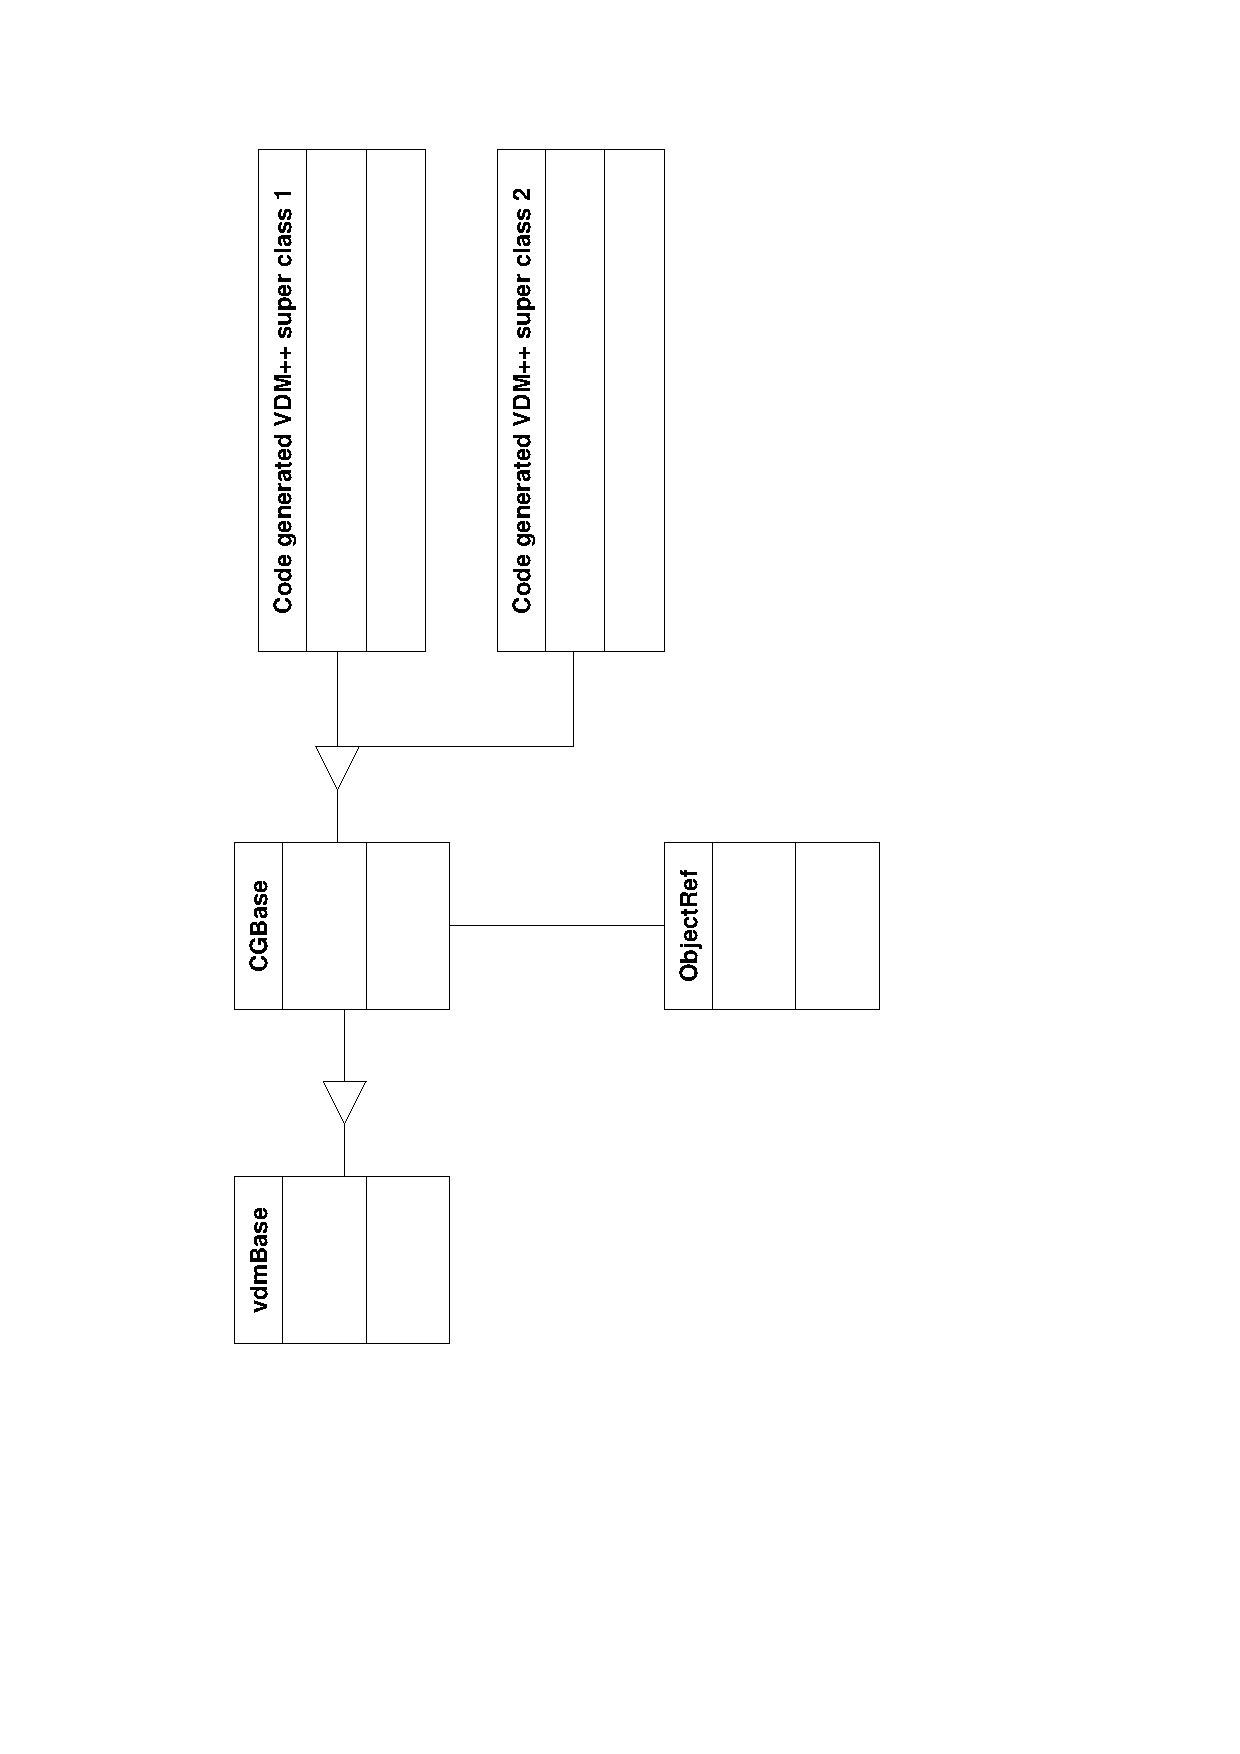
\includegraphics{cgbase}}}
    \caption{C++ クラス間の関係 \label{fig:cgb}}
  \end{center}
\end{figure}


%\insertfig{cgbase}{8cm}{Relation between C++
%  classes}{\label{fig:cgb}}



\subsection*{例題}

以下の $VDM^{++}$ クラスを考えよう:

\begin{verbatim}
class A

operations
  public Test: () ==> nat
  Test()  == 
    let a = 10 + 10 in 
      return a

end A
\end{verbatim}

以下のヘッダーファイル、 {\tt A.h}、は {\it VDM++ to C++ Code Generator\/}によって生成されている:

\begin{alltt}
{#ifndef _A_h}
{#define _A_h}

{#include <math.h>}
{#include "metaiv.h"}
{#include "cg.h"}
{#include "cg_aux.h"}
{#include "CGBase.h"}
{#include "A_anonym.h"}

class type_ref_A : public virtual ObjectRef \{
public:
  type_ref_A () : ObjectRef() \{\}
  type_ref_A (const Generic &c) : ObjectRef(c) \{\}
  type_ref_A (vdmBase * p) : ObjectRef(p) \{\}

  const wchar_t * GetTypeName () const \{
  return L"type_ref_A";
  \}
\};

class vdm_A : public virtual CGBase \{
friend class init_A ;
public:

vdm_A * Get_vdm_A () \{
  return this;
\}

ObjectRef Self () \{
  return ObjectRef(Get_vdm_A());
\}

int vdm_GetId () \{
  return VDM_A;
\};

vdm_A ();
virtual ‾vdm_A () {}
public:
  virtual Int vdm_Test ();
\};

{#endif}
\end{alltt}

これで以下の方法により、 {\tt A}型のオブジェクト参照を実装するために ObjectRef を用いることができる:

\begin{alltt}
{#include <iostream>}
{#include "A.h"}

int main ()
\{ 
  Sequence sq; Int i (10);
  ObjectRef cls1 (new vdm_A());
  ObjectRef cls2 (new vdm_A());

  sq.ImpAppend (i).ImpAppend (cls1).ImpAppend (cls2);

    wcout << VDM_A << " is the value of VDM_A" << endl;
    wcout << sq.ascii () << " is the value of sq" << endl;

  ObjectRef cls3 (sq[2]);
  if (cls3.MyObjectId () == VDM_A) \{ 
    vdm_A* cp = ObjGet_vdm_A(cls3);
    wcout << cp->vdm_Test ().ascii () << " is the result of Test ()" << endl;
    wcout << (cls1) == (cls2) << " is the result of cls1 == cls2" << endl;
    wcout << (cls1) == (cls3) << " is the result of cls1 == cls3" << endl;
  \}
  else
    wcout << "Something strange happened!" << endl;
    
  return 0;
\} 
\end{alltt}


\noindent このプログラムの実行結果は次の通り :

\begin{verbatim}
0 is the value of VDM_A
[ 10,@(0, 0x808dde4),@(0, 0x808debc) ] is the value of sq
20 is the result of Test ()
0 is the result of cls1 == cls2
1 is the result of cls1 == cls3
\end{verbatim}



\subsection{Generic}

{\tt Generic} は以下の要素関数をサポートする:

\vspace{0.5cm}

\begin{description}
\item[{\tt Generic G}] \mbox{}\\
      {\tt Generic}型の値として {\tt G} を宣言する。値は GenericValのインスタンスである。

     結果型 : {\bf void}

\item[{\tt Generic G(A)}] \mbox{}\\
      {\tt G} を、 {\tt A}の値と等しい{\tt Generic} 型の値として宣言する。

     結果型 : {\bf void}

\end{description}     

\section{集合型、列型、写像型}\label{templates}

集合、列、写像の型に対しては、相当する C++ テンプレートがある。
これらテンプレートを用いることで、さらに適切な型情報の型宣言を行うことが可能となる。
これらの型を用いると、集合だけでなく集合が含めることが可能な値型も宣言することができる。

\subsection{集合型}

 {\tt SET} テンプレートは {\tt Set} クラスから派生する。

 {\tt SET} テンプレートはコンストラクタ関数をサポートする:

\begin{description}
\item[{\tt SET<A> St}] \mbox{}\\
{\tt St} を {\tt A}型の{\tt Set}として宣言する。  {\tt St} の値は空集合に初期化される。

結果型: {\bf void}

\item[{\tt SET<A> St(St1)}] \mbox{} \\
 {\tt St} を{\tt A}型の {\tt Set}として宣言する。  {\tt St} の値は {\tt St1}の値に初期化される。

結果型: {\bf void}

\end{description}

加えて {\tt Set}クラスに作用する同等の関数や操作も {\tt SET} テンプレートに対して宣言される。

\subsection{列型}

 {\tt SEQ} テンプレートは {\tt Sequence} クラスから派生する。

 {\tt SEQ} テンプレートはコンストラクタ関数をサポートする:

\begin{description}
\item[{\tt SEQ<A> Sq}] \mbox{}\\
 {\tt Sq} を {\tt A}型の {\tt Sequence} として宣言する。 {\tt Sq} の値は空列に初期化される。

結果型: {\bf void}

\item[{\tt SEQ<A> Sq(Sq1)}] \mbox{} \\
 {\tt Sq} を{\tt A}型の {\tt Sequence} として宣言する。 {\tt Sq} の値は {\tt Sq1}の値に初期化される。

結果型: {\bf void}

\end{description}

加えて、 {\tt Sequence}クラスに作用する同等の関数や操作も {\tt SEQ} テンプレートに対して宣言される。

\subsection{写像型}

 {\tt MAP} テンプレートは {\tt Map} クラスから派生する。

 {\tt MAP} テンプレートはコンストラクタ関数をサポートする:

\begin{description}
\item[{\tt MAP<A,B> M}] \mbox{}\\
 {\tt M} を {\tt A} 型から {\tt B}への{\tt Map}として宣言する。 {\tt M} の値は空写像に初期化される。

結果型: {\bf void}

\item[{\tt MAP<A, B> M(M1)}] \mbox{} \\
 {\tt M} を {\tt A} 型から {\tt B}への{\tt Map}として宣言する。{\tt M} の値は {\tt M1}の値に初期化される。

結果型: {\bf void}

\end{description}

加えて、 {\tt Map} クラスに作用する同等の関数や操作も {\tt MAP} テンプレートのために宣言されている。



\section{エラーメッセージ} \label{error-messages}
エラーがライブラリ関数によって検出された場合、m4err ストリームに、エラーを検出したライブラリ関数を記述する文字列と共にエラー番号が 書かれる。 
その後プログラムを終了するために 'exit' 関数が呼び出される。

エラーは2つのカテゴリに分けられてきた。
ユーザーエラー (U) はライブラリの通常使用の下でおきる可能性がある。
例としては、空集合から要素を抽出しようとした場合である。 

内部エラー (I) はさらに重大なエラーである。 
これらのエラーは、ライブラリの通常使用の下では現れるはずのないものである。

\vspace{0.5cm}
\noindent

\begin{tabular}{|r|l|p{5.5cm}|c|} \hline
{\em No.} & {\em 記号名} & {\em 説明} 
           & {\em エラー型} \\ \hline \hline
1   & {\tt ML\_CONFLICTING\_RNGVAL} & 異なる値域値が既に存在する写像へのキーの挿入&U\\
2   & {\tt ML\_NOT\_IN\_DOM} & 写像に対し定義域中にないキーの適用&U\\
3   & {\tt ML\_CAST\_ERROR} & 汎用型の誤った型へのキャスト&U\\
4   & {\tt ML\_INDEX\_OUT\_OF\_RANGE} & 列、組、レコードの関数における範囲外のインデックス&U\\
5   & {\tt ML\_OP\_ON\_EMPTY\_SEQ} & 空列に対する違法な関数呼び出し&U\\
6   & {\tt ML\_OP\_ON\_EMPTY\_SET} & 空集合に対する違法な関数呼び出し&U\\
7   & {\tt ML\_NOT\_IN\_SET} & 集合に存在しない要素を取り除こうとした&U\\
8   & {\tt ML\_ASSIGN\_ERROR} & 異なる型の2変数間で代入をしようとした&U\\
9   & {\tt ML\_TRAVERSE\_CONFLICT} & 要素関数Nextを評価しているときに検出されたエラー&I\\
10  & {\tt ML\_HD\_ON\_EMPTY\_SEQUENCE} & 空列で hd を取り出そうとした&U\\                      
11  & {\tt ML\_TL\_ON\_EMPTY\_SEQUENCE} & 空列で tl を取り出そうとした&U\\
12  & {\tt ML\_RANGE\_ERROR} & 組やレコードに対する範囲外のインデックス&U\\                                                   
13  & {\tt ML\_ZERO\_REFCOUNT} & ゼロ参照カウンタの検出&I\\
14  & {\tt ML\_NULL\_REF} & ゼロポインタ参照&I\\\hline
15  & {\tt ML\_DIV\_BY\_ZERO} & ゼロによる除算 & U \\ \hline 
\end{tabular}


\bibliographystyle{iptes}
\bibliography{ifad}

 
\appendix
\section{ファイル} \label{files}
VDM C++ ライブラリへのインターフェイスは以下のファイルから構成される:

\begin{description}
\item[metaiv.h] は、第 \ref{specific-op}章で述べたすべての型の特有関数のプロトタイプを含むヘッダーファイルである。
  \item[vdm.lib](Windows)は、本書で述べた全関数の実装を含むアーカイブライブラリである。 
\item[libvdm.a](Mac、Linux) は、本書で述べた全関数の実装を含むアーカイブライブラリである。
\end{description}

\end{document}
